\section{Weak recovery with Generalized Linear Models} \label{2406:app:sec:weakrecoveryglm}
In this section, we restrict our analysis to matching architectures with \(p=k=1\), i.e. \emph{Generalized Linear Models} (GLMs). Moreover, we consider as activation function the Hermite polynomials \(\sigma = \text{He}_\ell\), so that we can have control on the information exponent of the problem.
Finally, the training algorithm is \emph{projected SGD}, given by Equation~\eqref{2406:eq:main:projected_sgd}.
We will also assume that \(a=a_\star=1\) throughout all the dynamics.

Let us start by noticing that the set of sufficient statistics reduces to just one single parameter \(m=\langle\vec w,\vec w_\star\rangle\).
Retracing backward all the steps of the Sections \ref{2406:sec:app:matching_architectures}~and~\ref{2406:sec:app:derivation_of_lb_equations} up to \eqref{2406:eq:app:generallowerbound}, we can obtain the lower bound for the update of \(m\). As examples the explicit equation for \(\sigma = \text{He}_2\) is
\[\begin{split}
    m_{t+1}-m_t \ge& \gamma_0 d^{-\delta}\Bigg[4m_t - 4m_t^3 - d^{-\delta}\gamma_0\mathbf{1}_{\{\mu\neq0\}}\left(8m_t-8m_t^3\right) +\\ 
        &+d^{-\delta+1-\mu}\frac{\gamma_0}{n_0}\left(24m_t-24m_t^3+2m_t^2\Delta\right)\Bigg],
\end{split}\]
while for \(\sigma = \text{He}_3\) is
\[\begin{split}
    m_{t+1}-m_t \ge& \gamma_0 d^{-\delta}\Bigg[18m_t^2 - 18m_t^4 - d^{-\delta}\gamma_0\mathbf{1}_{\{\mu\neq0\}}\left(162m_t + 324m_t^4 - 162m_t^5\right) +\\ 
&+d^{-\delta+1-\mu}\frac{\gamma_0}{n_0}\left(-1728m_t - 648m_t^3 + 3348m_t^4-972m_t^5-9\Delta m_t^3\right)\Bigg]. 
\end{split}\]
In general, for an Hermite polynomial activation \(\text{He}_\ell\), the equation of the evolution of \(m\) around \(m=0\) is given by
\begin{equation} \label{2406:eq:app:m_expansion}
    m_{t+1}-m_t \ge d^{-\delta}\beta_\ell m^{\ell-1} %+ o_d\left((m^{\tau=0})^{\ell-1}\right) 
        -d^{-\delta} \left(d^{-\delta+1-\mu}\alpha_\ell + d^{-\delta}\mathbf{1}_{\{\mu\neq0\}}\phi_\ell   \right)m
        %+ \text{h.o.t.} %\quad\text{with}\quad \Delta t = d^{-\delta}
\end{equation}
where we fixed \(\gamma_0=n_0=1\) for simplicity; \(\alpha_\ell, \beta_\ell, \phi_\ell\) are constants. For computing the full equations for any generic \(\ell\), with the constants values, we refer to the Mathematica notebook published in the repository of this work.

At initialization, \(m_0 = \sfrac{1}{\sqrt{d}}\). The crucial observation is that a sufficient condition to escape initialization is to have equation~\eqref{2406:eq:app:m_expansion} being  \emph{expansive}, namely \(\Delta m>0\) for \(m\) close to zero. This can be true if and only if \(\left(d^{-\delta+1-\mu}\alpha_\ell + d^{-\delta}\mathbf{1}_{\{\mu\neq0\}}\phi_\ell   \right)m\) is negligible when compared to \(\beta_\ell m^{\ell-1}\), so that the equation for \(m\) is lower-bounded by
\begin{equation} \label{2406:eq:app:m_expansive}
     \frac{\Delta m}{\Delta t} \ge \beta_\ell m^{\ell-1} + \text{h.o.t} \quad\text{with}\quad \Delta t = d^{-\delta}
\end{equation}
Assuming that \(\gamma = o_d(1)\), the bound becomes tight and we can also derive some sharp characterization of the escaping time. By simple arguments on differential equations, we can claim that the order of magnitude of steps needed to escape the initial mediocrity is given by
\[
 T = \begin{cases}
     O_d\left(\frac{1}{\Delta t}\right) & \ell=1 \\
     O_d\left(\frac{\log m_0}{\Delta t}\right) & \ell=2 \\
     O_d\left(\frac{1} {m_0^{\ell-2}\Delta t}\right) & \ell\ge3 \\
 \end{cases},
\]
remembering that \(m_0=\sfrac{1}{\sqrt{d}}\) and \(\Delta t = d^{-\delta}\), these lead to
\begin{equation} \label{2406:eq:app:escapingtimes}
\log_d T \sim \begin{cases}
    \max(\delta,0) & \ell=1 \\
    \log\log d + \delta & \ell=2 \\
    \delta - 1 +\sfrac{\ell}{2} & \ell\ge3 \\
 \end{cases}.
\end{equation}

It's clear that to escape as fast as possible, we want \(\delta\) to be the smallest possible, or in other words, having the learning rate as large as possible. Obviously, \(\delta\) is constrained by the values that make equation~\eqref{2406:eq:app:m_expansive} true (or equivalently by the assumptions of the formal proof in Appendix~\ref{2406:sec:app:proofs}).
The phase diagram of the allowed value of \(\delta\) and \(\mu\) is summarized in Figure~\ref{2406:fig:app:deltamu_phasediagram}: the green region is where the equations for \(m\) is expansive, the red and the yellow region is where the equations in attractive, so there is no escaping, the purple region is where we can't do expansion because the learning rate is too large and the process diverge. Figure~\ref{2406:fig:cold_start_pd} in the main text shows the same result in terms of \(T\) and \(n_b\), when \(\ell\ge3\).%; Figure~\ref{2406:fig:app:pd_l12} is showing the same for the 
\begin{figure}
    \centering
    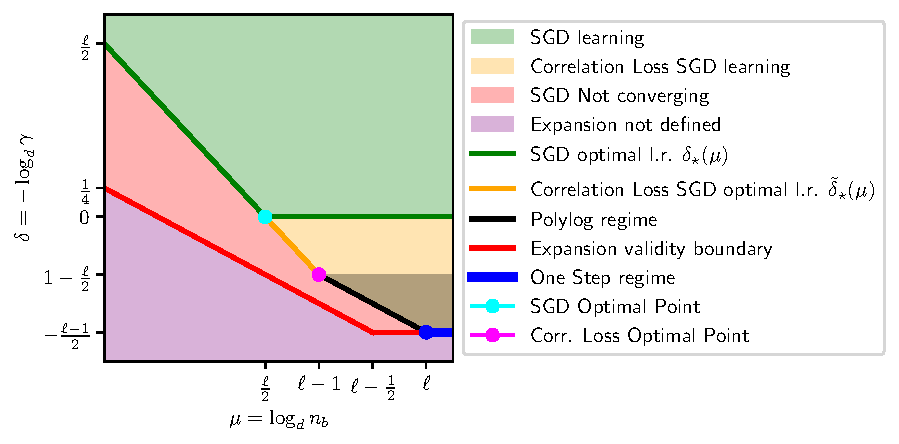
\includegraphics[width=0.9\textwidth]{figs/expansion_diagram}
    \caption{\textbf{Phase diagram for the learning rate:} The plot identifies different learning behaviors of standard SGD and \emph{Correlation Loss SGD} for different values of learning rate and batch size when considering randomly initialized networks, i.e. $m_0 = O(\sfrac{1}{\sqrt{d}})$.}
    \label{2406:fig:app:deltamu_phasediagram}
\end{figure}

\subsection{Correlations loss SGD}
When using \emph{Correlation Loss SGD}, Equation~\eqref{2406:eq:app:m_expansion} rewrite as 
\[
    \frac{\Delta m}{\Delta t} \ge \beta_\ell m^{\ell-1} %+ o_d\left((m^{\tau=0})^{\ell-1}\right) 
        -d^{-\delta+1-\mu}\alpha_\ell m
        %+ \text{h.o.t.}
\]
effectively removing a constraint on the possible values of \(\delta\). The modified version of SGD can use smaller values of \(\delta\) for escaping the initial condition, reaching regions in the phase diagram that are not allowed for SGD: this is colored in yellow in Figures~\ref{2406:fig:app:deltamu_phasediagram}~and~\ref{2406:fig:cold_start_pd}. Of course, if the learning rate becomes too large, all the theory does not work anymore (purple region in the diagram). In Figure~\ref{2406:fig:cold_start_pd} we show that the number of steps needed to weakly recover can be pushed down to be smaller than any power scaling with \(d\) (black and blue line on the x-axis). The picture becomes clearer if we look at the same diagram in terms of \((\mu,\delta)\): Correlation Loss SGD can be used with learning very large learning rates (\(1-\sfrac\ell2>\delta>-\sfrac{(\ell-1)}{2}\)) such that the escaping times is \(T=O(\mathrm{polylog}(d))\), as proved in Theorem~\ref{2406:thm:main:no_yhat_weak_recovery}.
We believe that the true number of steps is actually \(T=O(\mathrm{log}(d))\), but we could not find any formal proof; in Section~\ref{2406:app:sec:polylog}, we were able to show that for \(\ell=2\) we have \(T=O(\mathrm{log}(d))\), relying the result on numerical integration of our asymptotic theory. Lastly, if the learning rate is of order \(\gamma=O(d^{-\delta})=O(d^{\sfrac{\ell-1}{2}})\) we recover the result of \cite{dandi2023how}: the target can be weakly recovered in just one step, when the batch size is \(n_b>O(d^\ell)\).

\subsection{Simple example: retrieving \cite{arous2021online}}
In this section, we want to show how to find the same result presented in \cite{arous2021online} starting from our formalism.
There, online one-pass SGD is considered, meaning \(n_b=1 \implies \mu = 0\) in our context. Moreover, a vanishing learning rate is assumed, which implies \(\delta>0\), and all the bounds for the evolutions of \(m\) are tight. The condition for expansiveness of equation~\eqref{2406:eq:app:m_expansion} becomes
\[
m_0^{\ell-1} >> d^{-\delta+1}m_0 \implies (\ell-1)\log_d m_0 \ge -\delta + 1 + \log_d m_0 \implies \delta \ge 1 + (2-\ell)\log_d m_0
\]
Plugging in \(m_0 = \sfrac{1}{\sqrt{d}}\)  we finally get \(\delta \ge \sfrac{\ell}{2}\), where the equality is the best possible value of the learning rate in order to make the escaping faster. Note that for \(\ell=1\) we are also bounded from Lemma~\ref{2406:lem:app:boundongamma}, so \(\delta\ge1\). Combining with \eqref{2406:eq:app:escapingtimes}, finally gives us the the minimal number of steps needed
\begin{equation}
    T \sim \begin{cases}
        d & \ell =1 \\
        d\log d & \ell=2 \\
        d^{\ell-1} & \ell\ge3 \\
 \end{cases}.
\end{equation}
This result matches \cite{arous2021online}.
\subsection{Extension to $p>1$}
The extension to general two-layer network student functions ($p>1$), while keeping always the target fixed to be a single-index one, can be readily done by performing an analysis similar to the above. The considerations on the weak recovery trade-offs done in the previous sections are not changed upon re-scaling the learning rate with the hidden layer size $p=O(1)$, i.e. $\sfrac{\gamma_{\rm 2LNN}}{p} = \gamma_{\rm GLM}$. Therefore, the scaling laws detailed in the phase diagram (Fig.~\ref{2406:fig:cold_start_pd}) are not modified, and only prefactors, i.e. quantity not scaling with the input dimension, change with respect to the $p=1$ case. We illustrate this phenomenon numerically in Fig.~\ref{2406:fig:app:k1p4singleindex}. We leave the detailed theoretical analysis of the $p>1$ case for future work, with particular attention to the limit $p \to \infty$ which we believe is an interesting avenue of future research.


\begin{figure}
    \centering
    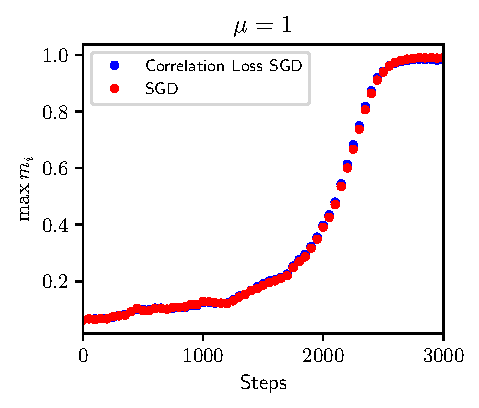
\includegraphics[width=.49\textwidth]{figs/singleidexteacher_widestudent_mu1}
    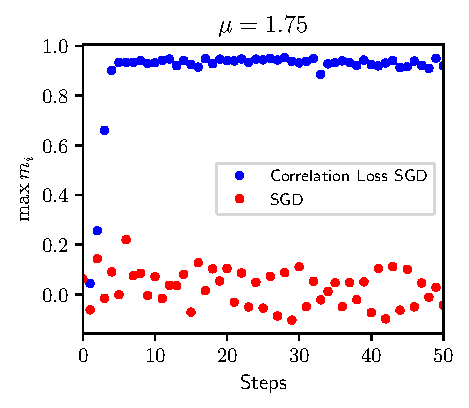
\includegraphics[width=.49\textwidth]{figs/singleidexteacher_widestudent_mu1.75}
    \caption{learning single-index teacher with a wide student, when information exponent is \(\ell=3\): \(f^\star(\vec{x})=\text{He}_3(\vec{w}^\star\cdot\vec{x}), f(\vec{x})=\sfrac14\sum_{i=1}^4\text{He}_3(\vec{w}_i\cdot\vec{x})\).
    Our theory extends to this case, showing that when \(\mu>\sfrac\ell2\) only correlation loss can weakly recover the target.
    (\(d=256, \gamma = \gamma_0\cdot p n_b d^{-\sfrac\ell/2}\))
    }
    \label{2406:fig:app:k1p4singleindex}
\end{figure}
